\begin{figure}[b!]
    \centering
    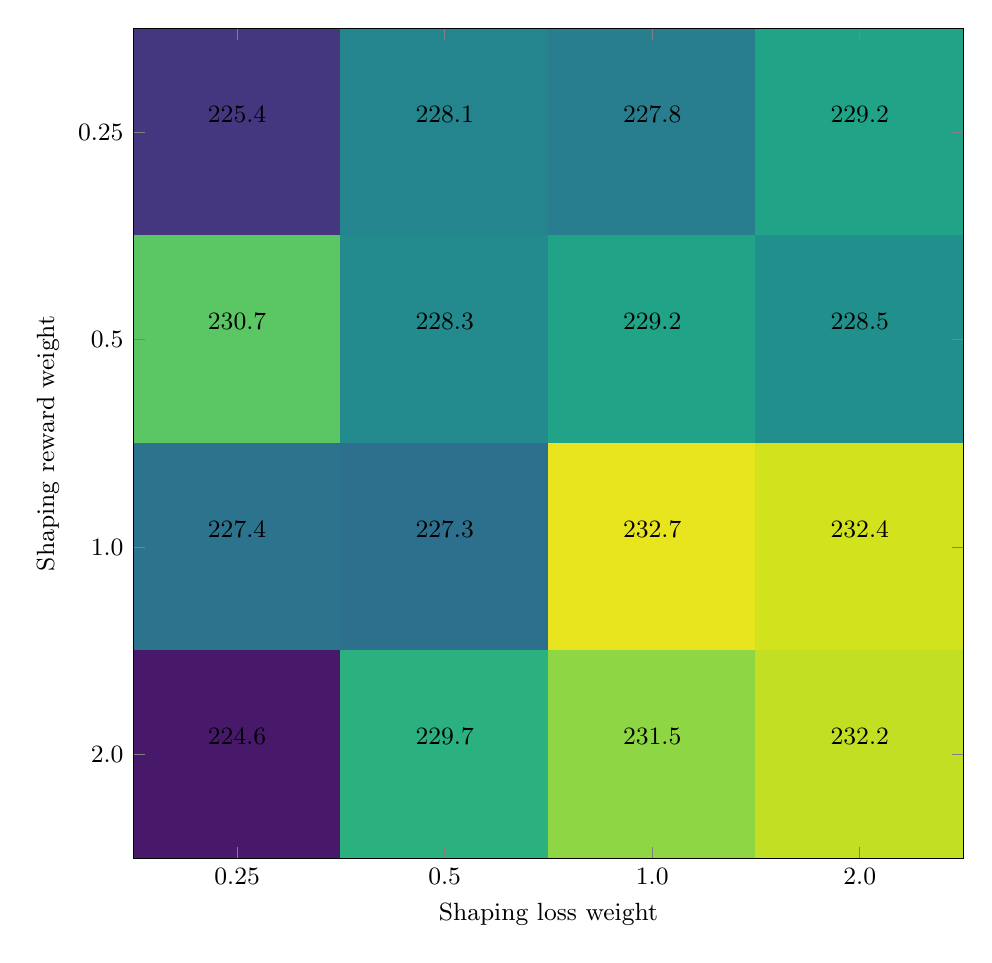
\begin{tikzpicture}
        \begin{axis}[
                width=\columnwidth,
                height=\columnwidth,      % square plot
                axis equal image,
                xmin=0.5, xmax=4.5,       % 4x4 grid with full cells visible
                ymin=0.5, ymax=4.5,
                enlargelimits=false,
                xlabel={Shaping loss weight},
                ylabel={Shaping reward weight},
                colormap/viridis,
                xlabel style={font=\small},
                ylabel style={font=\small},
                title style={font=\small},
                xtick={1,2,3,4},
                xticklabels={0.25, 0.5, 1.0, 2.0},
                ytick={1,2,3,4},
                yticklabels={0.25, 0.5, 1.0, 2.0},
                xticklabel style={font=\small},
                yticklabel style={font=\small},
                point meta min=224,
                point meta max=233,
                nodes near coords,
                nodes near coords style={font=\small, color=black},
                every node near coord/.append style={xshift=0pt, yshift=0pt},
            ]

            % use integer grid coords so cells are uniform
            \addplot[
                matrix plot,
                mesh/cols=4,
                point meta=explicit
            ] table[row sep=\\,meta=score] {
                    x  y  score \\
                    1  1  225.4 \\
                    1  2  230.7 \\
                    1  3  227.4 \\
                    1  4  224.6 \\
                    2  1  228.1 \\
                    2  2  228.3 \\
                    2  3  227.3 \\
                    2  4  229.7 \\
                    3  1  227.8 \\
                    3  2  229.2 \\
                    3  3  232.7 \\
                    3  4  231.5 \\
                    4  1  229.2 \\
                    4  2  228.5 \\
                    4  3  232.4 \\
                    4  4  232.2 \\
                };

        \end{axis}
    \end{tikzpicture}
    \caption{Shaping parameters ablation}
    \label{fig:shaping-heatmap}
\end{figure}
